\chapter[Referencial Teórico]{Referencial Teórico}

\section{Considerações Iniciais}

Neste capítulo, são apresentadas as bases teóricas para a elaboração do aplicativo com o objetivo de facilitar o entedimento dos termos utilizados. O capítulo está estruturado em seções. Na seção 2.1 será descrito tudo sobre o ciclo menstrual feminino, na seção 2.2 será apresentado os conceitos da produtividade, como medi-la e como melhora-la, na seção 2.3 serão apresentados os possíveis perfis das mulheres com base no ciclo menstrual e na seção 2.4 será abordada o sistema de recomendação.

\section{O Ciclo Mentrual}

O ciclo menstrual é um fenômeno biológico que ocorre em mulheres saudáveis na qual a carecterística nótavel é o fluxo sanguíneo vaginal\cite{guyton2012}. Ele é ciclico e ocorre como resultado direto de variações das concentrações hormonais secretadas pelo eixo hipotálamo-hipófise-gonadal. Estudos sugerem que essas flutuações hormonais, principalmente de estrogênio e progesterôna, que ocorrem no decorrer do ciclo, podem influenciar as emoções, comportamento e cognição das mulheres \cite{poroma2014}, afetando diretamente o seu dia-a-dia, como por exemplo, a performance nas tarefas cotidianas ou relacionamentos interpessoais.

O ciclo ideal tem como base 28 dias e por convenção o primeiro dia de menstruação é a marca do início do ciclo e a marca do final do ciclo anterior, caso não tenha ocorrido a gravidez. O ciclo pode ser dividido em duas fases, a fase folícular e a fase lútea, o períoodo da menstruação está presente no início da fase folícular e o período da ovulação está situada entre as duas fases. Mais informações sobre as fases, quanto tempo elas duram, quais hormônios atuam, e a influência deles nas mulheres, serão pontuadas nas subseções seguintes. 

 
\subsection{Fase Folicular}

A fase folicular é a primeira fase do ciclo menstrual, começa com o inicio da menstruação e termina com a ovulação. Enquanto ocorre a menstruação e os hormônios estimulante dos ovários(principalmente FSH) estão em concentração baixa, a fase é referida como fase folicular inicial.

Essa é a fase responsável pelo desenvolvimento de folículos dos quais um será selecionado e se transformará em um óvulo(corpos lutem) e dará início a ovulação. Os folículos se desenvolvem em resposta ao aumento do hormônio folícul-estimulante (FSH)\lq\lq (Fig. \ref{fig01})  e assim que um deles é selecionado, o FSH diminui gradativamente e progressivamente a produção de estrogénios começão a aumentar. Os estrogénios produzidos pelo folículo em crescimento são responsáveis também pelo desenvolvimento do endométrio e essa fase é normalmente referido como fase folicular tardia.

Normalmente, mulheres de 18 a 24 anos com ciclo de 28 dias tem a fase com o comprimento de 14 dias e mulheres de 40 a 44 anos tem de 10 dias \cite{lenton1984a}, o que indica a diminuição progressiva do tamanho da fase folicular com o avanço da idade. Em mulheres jovens a diferença no tamanho do ciclo é normalmente provocada por ciclo mais curtos ou mais longos na fase folicular \cite{lenton1984a}. Ciclos inrregulares também costumam ser pela variação no tamanho da fase folicular, enquanto a fase lútea segue normalmente com tamanho fixo de 14 dias. Então, em um ciclo de 28 dias a fase folicular tem 14 dias e em um ciclo de 30 ele teria 16 dias.

\begin{figure}[h]
	\centering
	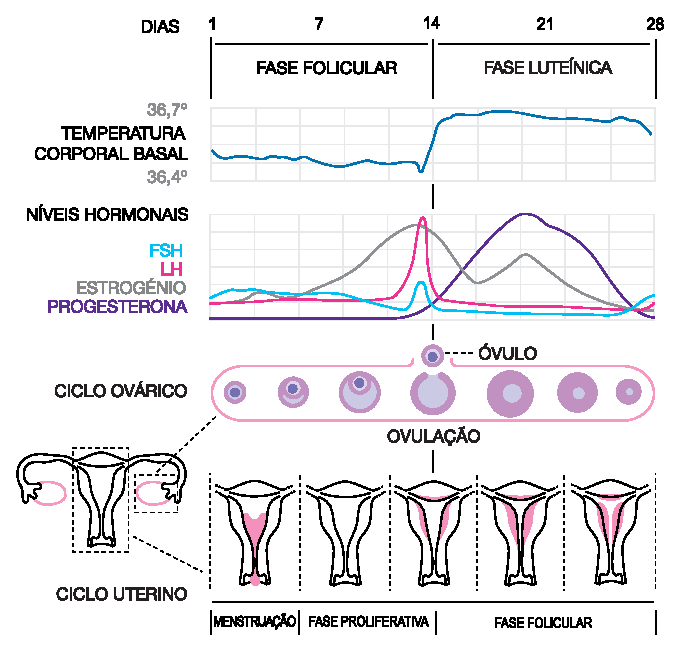
\includegraphics[keepaspectratio=true,scale=0.8]{figuras/MenstrualCycle2_pt.eps}
	\caption{Ciclo Menstrual}
        \label{fig01}
\end{figure}

Ápos passar a menstruação, mulheres relataram sentir alterações de humor, comportamentais e sintomas físicos. Esses sintomas variam entre melhoras na pele e no cabelo,perca de peso, diminuição na sensação de inchaço, diminuição ou aumento na líbido, humor mais estável, autoestima elevada, sensação de liberdade, resistência a dor,  aumento na confiança, animação, foco, inspiração e na comunicação.

Na realização de atividades, algumas relataram que atividades como realizar atividade física, atividades ao ar livre, trabalho em equipe, reuniões, estudar, atividades domésticas e começar projetos novos costumam ser mais fáceis nessa fase. Não foram relatadas nenhuma difículdade em realizar outras tarefas.

\subsubsection{Menstruação}

A menstruação marca o início do ciclo menstrual e o fim do ciclo anterior e é caracterizada pelo fluxo sanguíneo vaginal. Ocorre quando não há fecundação no ciclo anterior e é composta por sangue e tecido uterino derivado da descamação das paredes internas do útero(endométrio). Normalmente dura cerca de 5 dias, mas pode variar demulher para mulher.

O fluxo do sangramento também varia muito, mas costuma ser mais intenso nos primeiros dias. O fluxo menstrual pode ser leve, moderado ou intenso.

Algumas mulheres relatam sentir alterações de humor, comportamentais e sintomas físicos durante a menstruação. Esses sintomas variam entre cólica, surgimento de espinhas, sensação de inchaço, retenção de líquido, seios doloridos, cansaço, inrritabilidade, indisposição, ansiosidade, fácil alteração de humor, dores no corpo, dores de cabeça, alterações no sono, estresse e baixa ou alta líbido.

Na realização de atividades, algumas relataram que atividade como exercícios físicos, lidar como pessoas, ir a faculdade, trabalhar e atividades presenciais se tornam mais difíceis de serem realizadas, enquanto tarefas como, dormir, ler e exercer atividade individuais, se tornam mais fáceis. Atividades como assistir filmes e séries, estudar e realizar atividades domésticas foram citadas nas duas categorias.

\subsection{Ovulação}

A ovulação em si não é uma fase, propriamente dita, mas quando referida como tal carrega o significado de um período estimado em que há a possível liberação do óvulo e maior probabilidade de gravidez. A fase também é referida como fase fértil e neste estudo é dividida das outras fases por sua importância.

A ovulação acontece pelo equilíbrio entre vários hormonios. Clinicamente é possível determinar o ciclo ovulatório pelo surgimento do LH e a secreção de progesterona da fase lútea \cite{fritz2010}.Quando o estradiol chega ao pico, de 12 a 14 horas depois o LH surge e de 10 a 12 horas depois, faz com que o ovócito complete a sua maturação, rompendo o folículo e sendo libertado na cavidade abnominal onde se dirige à trompa de Falópio \cite{fritz2010}. A subida do LH é o que determina o início da fase lútea.

Como através de um aplicativo não é possível medir o aparecimento do LH para determinar o fim da fase folicular e o início da ovulação e a ovulação é estimada através de uma janela então a ovulação e a fase folicular acabarão se sobrepondo nesse estudo.

A detecção da ovulação costuma ser difícil, mas algumas mulheres relatam sentir alterações de humor, comportamentais e sintomas físicos durante a ovulação. Esses sintomas variam entre aumento na líbido, fisgadas ou dores no abdômen perto do ovário, mais disposição para trabalhar e estudar, aumento nos seios, melhora na pele ou aparições de espinhas.

Na realização de atividades, algumas relataram que atividade como trabalhar, estudar e socializar. Se concentrar e realizar atividades físicas foram citadas nas categorias mais fáceis ou mais difíceis.

\subsection{Fase Lútea}

Com o evento da ovulação, o folículo se transforma em um corpo lúteo e as células das paredes do folículo começam a produção de progesterona para preparar o endométrio para a chegada do óvulo no caso de concepção. O pico da progesterona se dá normalmente por volta do vigésimo primeiro dia do ciclo \cite{nikas2003}. Caso não haja fecundação, a progesterona decai progressivamente e causa novamente a menstruação, continuando assim o ciclo.

A fase lútea tem duração de 14 dias e costuma ser constante nas mulheres, sem grande variação, mesmo que o tamanho do ciclo varie.É comum no final dessa fase, no período que antecede a menstruação, a aparição da tensão pré menstrual.

\subsubsection{Tensão Pré Menstrual}

\subsection{Método Baseado em Calendário}

Apesar de na literatura sobre fertilidade, o método preferido para capturar a fase do ciclo menstrual ser medidas diárias dos níveis de hormônios combinados ao ultrassom vaginal para acompanhar o desenvolvimento folicular \cite{ecochard2001} ou a combinação de medidas hormonais, temperatura corporal Basal e o método baseado em calendário \cite{becker2005} o aplicativo tem a limitação de não poder realizar medidas hormonais, nem ultrassons e não pode contar sempre com a TCB da sua usuária, portanto o método escolhido para classificar as fases do ciclo foi o método baseado em calendário.

Nesse método, uma contagem através do calendário é usada para determinar a fase do ciclo. O auto-relato do primeiro dia de menstruação é utilizado como ponto inicial do calendário e as fases são determinadas contando-se \lq \lq n\rq \rq  números de dias para frente ou de de trás para frente a partir da data de ínicio privestia para o próximo ciclo \cite{wideman2013}.

O ciclo base utilizado é normalmente o de 28 dias e para representar eventos ovulatórios(próximo a altos níveis de estradiol, antes de um aumento significativo da progesterona) é contado 10 a 14 dias a partir do início do ciclo ou de 12 a 14 dias a partir do dia de previsão para início do próximo ciclo, mas enquanto os eventos ovulatórios ocorrem em média entre esses dias o momento real da ovulação pode variar significativamente a partir desta janela. O méio da fase lútea em que os hormônios ficam estábilizados normalmente é contado de 17 a 21 dias do início do ciclo ou de 7 a 9 dias a partir do final do ciclo \cite{wideman2013}. A \lq\lq Figura \ref{fig02}\rq\rq\ representa um ciclo de 28 dias.

Como normalmente a diferença de tamanho dos ciclos se dá por um aumento no tamanho da fase folícular \cite{lenton1984a}, para ciclos maiores ou menores que 28 dias a ovulação é adiantada ou atrasada pela diferença entre o tamanho do ciclo e o ciclo base de 28 dias. Por exemplo, se for um ciclo de 32 dias, a ovulação provavelmente ocorrerá entre o 14 e 18 dia a partir do ínicio do ciclo.

\begin{figure}[h]
	\centering
	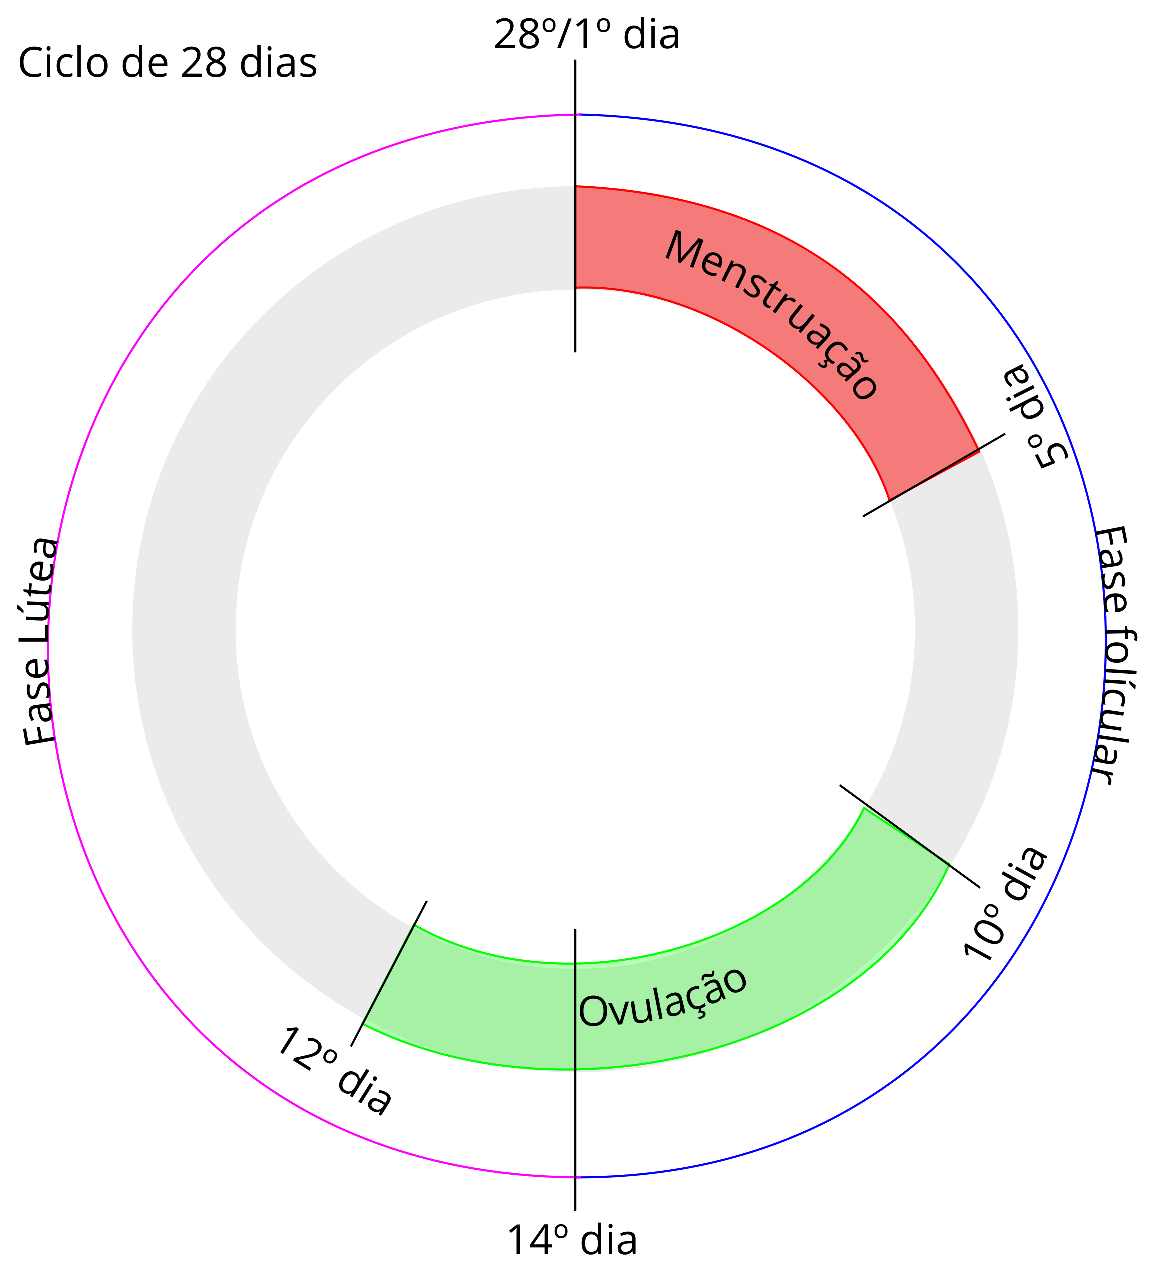
\includegraphics[keepaspectratio=true,scale=0.3]{figuras/calendario.eps}
	\caption{Calendário do ciclo menstrual e suas fases}
        \label{fig02}
\end{figure}

\subsection{Influências no ciclo menstrual}

\subsubsection{Métodos Contraceptivos}

\subsubsection{Disturbios hormonais}

\section{Perfil das mulheres}

\section{Sistema de Recomendação}

\section{Considerações Finais do Capítulo}

